\documentclass[12pt]{article}

\usepackage[margin=1in]{geometry}
\usepackage{amsmath}
\usepackage{amssymb}
\usepackage{booktabs}
\usepackage{float}
\usepackage{graphicx}
\usepackage{subcaption}
\usepackage{xcolor}

\graphicspath{{figures/}}

\newcommand{\studentname}{KARTHIKEYAN M}
\newcommand{\registernumber}{26120004}
\newcommand{\teammatename}{MIRTHULA R}
\newcommand{\teammateregister}{261200121}
\newcommand{\submissionmonth}{SEPTEMBER 2026}

% Replace every red prompt with your own explanation before submission.
\newcommand{\todo}[1]{%
  \par\noindent
  \textcolor{red}{\textbf{[WRITE HERE:} \textit{#1}\textbf{]}}
  \par
}

\begin{document}

\begin{titlepage}
\centering
\vspace*{2cm}
{\Large \textbf{ASSIGNMENT REPORT-4}}\\[2cm]

\textbf{Submitted by :}\\[0.3cm]
\textbf{\studentname} \ [\registernumber]\\[0.3cm]
\textbf{\teammatename} \ [\teammateregister]\\[2cm]

\textbf{Under the guidance of :}\\[0.3cm]
\textbf{HEMA ARUNACHALAM MURTHY}\\[1.5cm]

\textbf{For The Subject}\\[0.5cm]
{\Large \textbf{Pattern Recognition and Machine Learning}}\\[0.3cm]
\textbf{(26AI5707)}\\[3cm]

\vfill
\textbf{DEPARTMENT OF COMPUTER SCIENCE \& ENGINEERING}\\[0.3cm]
\textbf{SHIV NADAR UNIVERSITY}\\[0.3cm]
\textbf{KALAVAKAM}\\[1.5cm]
\textbf{\submissionmonth}
\end{titlepage}

\section*{INTRODUCTION}

The assignment's whole idea is about how covariance matrix controls the geometry of a 2D Gaussian Distribution. We start with generating normal data and move into experimenting with different covariance matrices such as isotropic, diagonal, full covariance matrices and visualize the contours of the 2D Gaussian (i.e.) Constant density curves and to finish it all up we create 2 gaussian classes and experiment with different covariance matrices to explore the difference in decision boundaries we get.

\section*{MATHEMATICAL BACKGROUND}

For a $d$-dimensional Gaussian random vector, the probability density looks something like this.

\begin{equation}
  p(\mathbf{x}) =
  \frac{1}{(2\pi)^{d/2}|\boldsymbol{\Sigma}|^{1/2}}
  \exp\left(
    -\frac{1}{2}
    (\mathbf{x}-\boldsymbol{\mu})^{\mathsf T}
    \boldsymbol{\Sigma}^{-1}
    (\mathbf{x}-\boldsymbol{\mu})
  \right).
  \label{eq:multivariate-gaussian}
\end{equation}

Here, the quadratic term

\begin{equation}
  d_M^2(\mathbf{x},\boldsymbol{\mu}) =
  (\mathbf{x}-\boldsymbol{\mu})^{\mathsf T}
  \boldsymbol{\Sigma}^{-1}
  (\mathbf{x}-\boldsymbol{\mu})
  \label{eq:mahalanobis}
\end{equation}

is the squared Mahalanobis distance. The constant density curves are plotted by taking a constant value for this expression.

\begin{equation}
  (\mathbf{x}-\boldsymbol{\mu})^{\mathsf T}
  \boldsymbol{\Sigma}^{-1}
  (\mathbf{x}-\boldsymbol{\mu}) = c.
  \label{eq:constant-density}
\end{equation}

Here we use Mahalanobis distance because if we had used euclidean distance, then it doesn't take the spread of different classes into account and it also doesn't consider the correlation between features and that might cause mis-classification when dealing with discrimination functions later. Because it would say a certain value is equally likely when they are clearly not when you take spread into picture.

\section*{EXPERIMENTAL SETUP}

The experiments starts by creating a $N=1000$ samples with a fixed random seed of 42. Two one-dimensional Gaussian samples are generated and then stacked as columns
to form the two dimensional samples. The initial parameters were

\begin{equation}
  \boldsymbol{\mu}=
  \begin{bmatrix}2\\4\end{bmatrix},
  \qquad \sigma=1.
\end{equation}

Gaussian samples are generated using Marsaglia polar method that was implemented in the lab1 and we also kept the seed fixed for reproducibility. After this we start working with a matrix $X$ of $(1000, 2)$ that contains gaussian features stacked as columns.

\section*{ISOTROPIC COVARIANCE MATRIX}

For the isotropic case, the target covariance matrix is

\begin{equation}
  \mathbf{C}=\sigma^2\mathbf{I}
  =\begin{bmatrix}1&0\\0&1\end{bmatrix}.
\end{equation}

The estimated mean and covariance are

\begin{equation}
  \hat{\boldsymbol{\mu}}=
  \begin{bmatrix}1.9841\\3.9676\end{bmatrix},
  \qquad
  \hat{\mathbf{C}}=
  \begin{bmatrix}
    1.0380 & 0.0463\\
    0.0463 & 1.0752
  \end{bmatrix}.
\end{equation}

\begin{figure}[H]
  \centering
  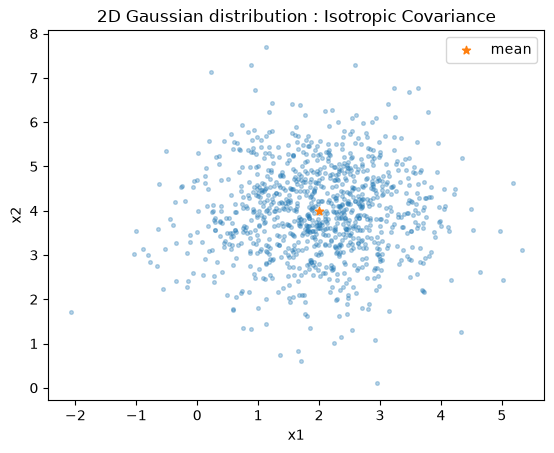
\includegraphics[width=0.70\textwidth]{isotropic_samples.png}
  \caption{Samples generated using isotropic covariance.}
  \label{fig:isotropic-samples}
\end{figure}

\begin{table}[H]
  \centering
  \caption{Theoretical and estimated eigenvalues for isotropic covariance.}
  \begin{tabular}{lccc}
    \toprule
    Direction & Theoretical $\lambda$ & Estimated $\lambda$ & Estimated axis length ($c=1$) \\
    \midrule
    Major & 1.0000 & 1.1065 & 2.104 \\
    Minor & 1.0000 & 1.0067 & 2.007 \\
    \bottomrule
  \end{tabular}
\end{table}

\begin{figure}[H]
  \centering
  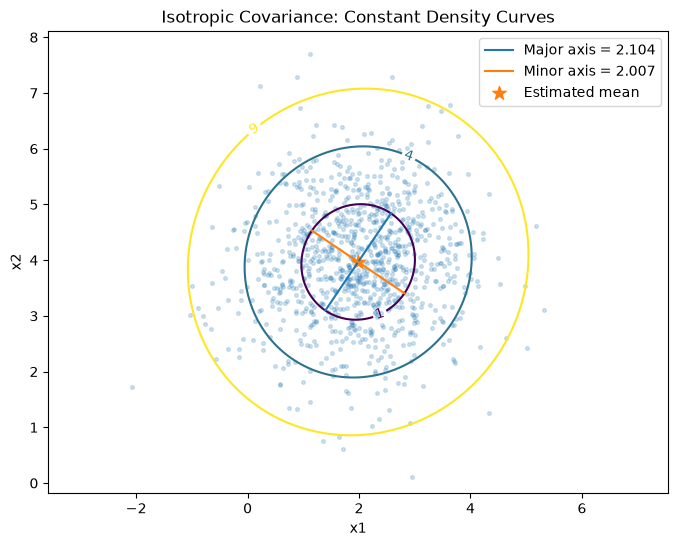
\includegraphics[width=0.82\textwidth]{isotropic_contours_axes.png}
  \caption{Constant Mahalanobis-distance curves and estimated principal axes
  for the isotropic data.}
  \label{fig:isotropic-contours}
\end{figure}

Here, theoretically we should have gotten the off-diagonals as zero. But we aren't getting it. Due to the fact that we are randomly generating data and there might be chance that the features we generated to correlate somewhat but, the off-diagonals aren't huge enough to make the tilt as expected and they form a circle for the contour because they have approximately equal variances.

\section*{DIAGONAL COVARIANCE MATRIX}

The target diagonal covariance was

\begin{equation}
  \mathbf{C}_{\mathrm{diag}}=
  \begin{bmatrix}4&0\\0&1\end{bmatrix}.
\end{equation}

Starting from the isotropic data, the transformation used is

\begin{equation}
  \mathbf{Y}=\boldsymbol{\mu}+
  \mathbf{C}_{\mathrm{diag}}^{1/2}
  (\mathbf{X}-\boldsymbol{\mu}),
  \qquad
  \mathbf{C}_{\mathrm{diag}}^{1/2}=
  \begin{bmatrix}2&0\\0&1\end{bmatrix}.
  \label{eq:diagonal-transform}
\end{equation}

The estimated covariance are

\begin{equation}
  \hat{\mathbf{C}}_{\mathrm{diag}}=
  \begin{bmatrix}
    4.1520 & 0.0927\\
    0.0927 & 1.0752
  \end{bmatrix}.
\end{equation}

\begin{table}[H]
  \centering
  \caption{Theoretical and estimated eigenvalues for diagonal covariance.}
  \begin{tabular}{lccc}
    \toprule
    Direction & Theoretical $\lambda$ & Estimated $\lambda$ & Estimated axis length ($c=1$) \\
    \midrule
    Major & 4.0000 & 4.1548 & 4.077 \\
    Minor & 1.0000 & 1.0724 & 2.071 \\
    \bottomrule
  \end{tabular}
\end{table}

\begin{figure}[H]
  \centering
  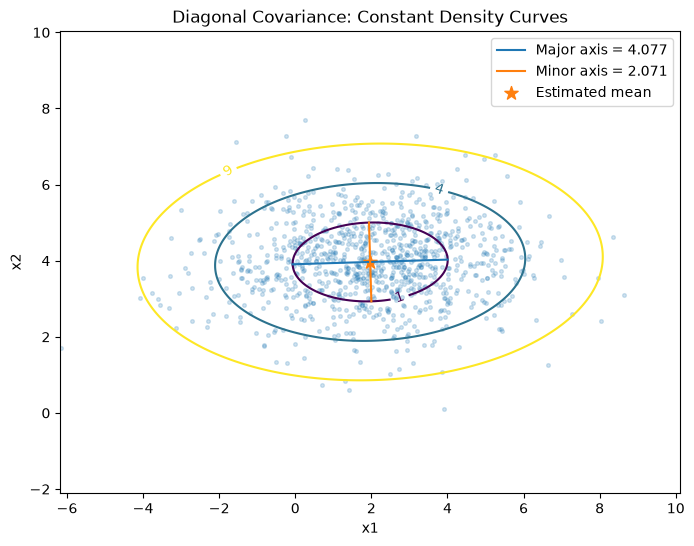
\includegraphics[width=0.82\textwidth]{diagonal_contours_axes.png}
  \caption{Constant density curves and principal axes for diagonal covariance.}
  \label{fig:diagonal-contours}
\end{figure}

Here the major axis has twice the spread compared to the minor axis. Due to the fact that it has more variance along that direction and thus forming a elliptical shape for the contours and also another thing to note here is that the principal axes are close to co-ordinate axes because we made it that way. According to the theoretical diagonal covariance matrix, there are no off-diagonals and variance of $x1$ is $4$ and $x2$ is $1$. As you can clearly see we intentionally made the variance along one axis large and another as $1$ and no off-diagonals so the contours doesn't tilt as well.

\section*{FULL COVARIANCE MATRIX}

The full covariance matrix was chosen as

\begin{equation}
  \mathbf{C}_{\mathrm{full}}=
  \begin{bmatrix}
    4.0 & 1.5\\
    1.5 & 1.0
  \end{bmatrix}.
\end{equation}

For a full covariance matrix, the element-wise square root is not the required
matrix square root. Using the eigendecomposition
$\mathbf{C}=\mathbf{Q}\boldsymbol{\Lambda}\mathbf{Q}^{\mathsf T}$, it was
constructed as

\begin{equation}
  \mathbf{C}^{1/2}=
  \mathbf{Q}\boldsymbol{\Lambda}^{1/2}\mathbf{Q}^{\mathsf T},
  \qquad
  \mathbf{C}^{1/2}(\mathbf{C}^{1/2})^{\mathsf T}=\mathbf{C}.
  \label{eq:matrix-square-root}
\end{equation}

The transformed samples had estimated covariance

\begin{equation}
  \hat{\mathbf{C}}_{\mathrm{full}}=
  \begin{bmatrix}
    4.2597 & 1.6625\\
    1.6625 & 1.1065
  \end{bmatrix}.
\end{equation}

\begin{table}[H]
  \centering
  \caption{Theoretical and estimated eigenvalues for full covariance.}
  \begin{tabular}{lccc}
    \toprule
    Direction & Theoretical $\lambda$ & Estimated $\lambda$ & Estimated axis length ($c=1$) \\
    \midrule
    Major & 4.6213 & 4.9744 & 4.461 \\
    Minor & 0.3787 & 0.3919 & 1.252 \\
    \bottomrule
  \end{tabular}
\end{table}

\begin{figure}[H]
  \centering
  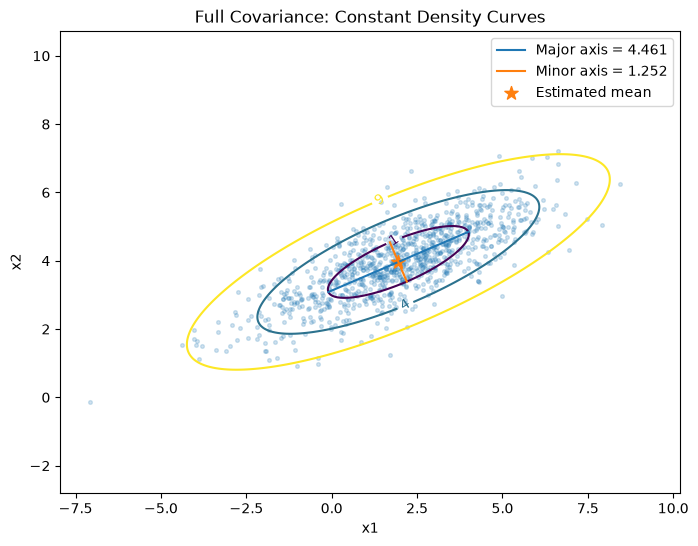
\includegraphics[width=0.82\textwidth]{full_contours_axes.png}
  \caption{Tilted constant density curves and principal axes for full
  covariance.}
  \label{fig:full-contours}
\end{figure}

Here, we have non-zero off-diagonals hence we expect the constant density curves to tilt a little bit corresponding to the covariance between $Cov(x1, x2)$. The estimated $Cov(x1, x2)$ is $1.6$ (+ve) and hence, $x2$ tend to increase as $x1$ increases (i.e.) positive tilt and also another thing to note here is that we have large variance on major axis and lesser variance on the minor axis. Thus a elliptical contour with a tilt.

\section*{TWO GAUSSIAN CLASSES}

For equal class priors, the class-dependent part of the Gaussian discriminant
function is

\begin{equation}
  g_i(\mathbf{x})=
  -\frac{1}{2}\log|\boldsymbol{\Sigma}_i|
  -\frac{1}{2}
  (\mathbf{x}-\boldsymbol{\mu}_i)^{\mathsf T}
  \boldsymbol{\Sigma}_i^{-1}
  (\mathbf{x}-\boldsymbol{\mu}_i).
  \label{eq:discriminant}
\end{equation}

The decision boundary contains all points satisfying

\begin{equation}
  g_1(\mathbf{x})-g_2(\mathbf{x})=0.
  \label{eq:decision-boundary}
\end{equation}

\subsection*{Equal covariance matrices}

The first experiment used

\begin{equation}
  \boldsymbol{\mu}_1=\begin{bmatrix}0\\0\end{bmatrix},
  \quad
  \boldsymbol{\mu}_2=\begin{bmatrix}4\\4\end{bmatrix},
  \quad
  \boldsymbol{\Sigma}_1=\boldsymbol{\Sigma}_2=\mathbf{I}.
\end{equation}

\begin{figure}[H]
  \centering
  \begin{subfigure}[t]{0.48\textwidth}
    \centering
    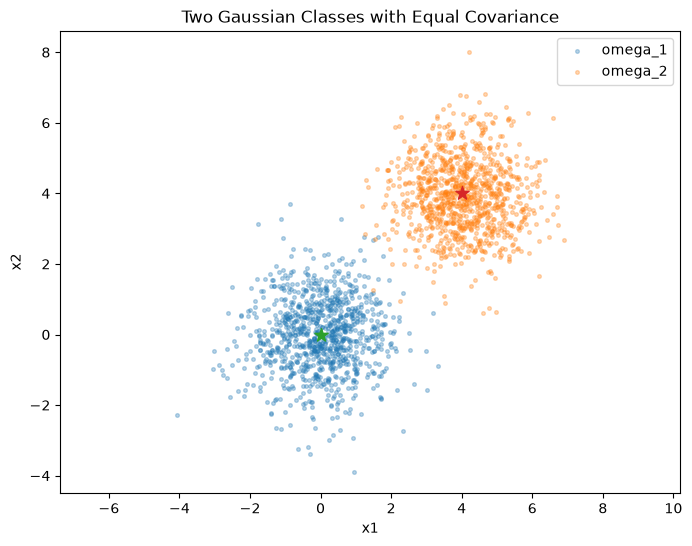
\includegraphics[width=\textwidth]{equal_covariance_samples.png}
    \caption{Generated class samples.}
  \end{subfigure}
  \hfill
  \begin{subfigure}[t]{0.48\textwidth}
    \centering
    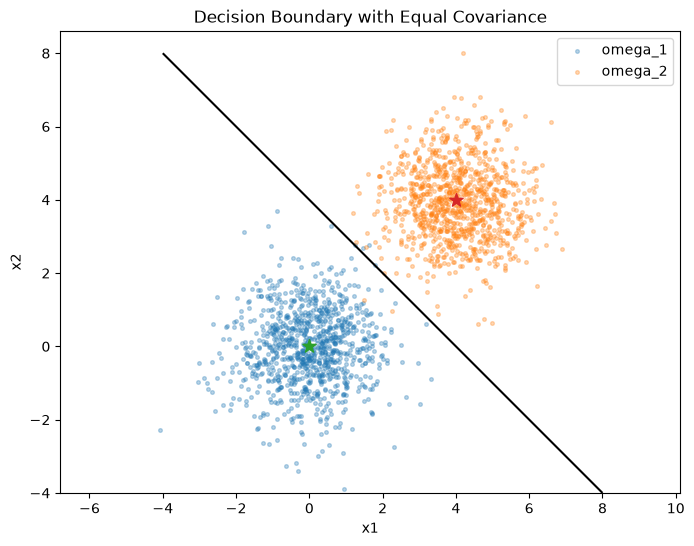
\includegraphics[width=\textwidth]{equal_covariance_boundary.png}
    \caption{Resulting decision boundary.}
  \end{subfigure}
  \caption{Two Gaussian classes with equal covariance matrices.}
  \label{fig:equal-covariance-classes}
\end{figure}

Here, since both the classes have the same covariance matrix. The quadratic terms cancel out in the discrimination function and thus leaving out a linear boundary and another thing is the boundary appears mid-way between the means of different classes and that would be $(2, 2)$ in this case. This is because they data points of each class have exact same covariance but just centered in different locations that's it.

\subsection*{Different covariance matrices}

The second experiment retained the same means but used

\begin{equation}
  \boldsymbol{\Sigma}_1=
  \begin{bmatrix}1&0\\0&1\end{bmatrix},
  \qquad
  \boldsymbol{\Sigma}_2=
  \begin{bmatrix}4&1.5\\1.5&2\end{bmatrix}.
\end{equation}

\begin{figure}[H]
  \centering
  \begin{subfigure}[t]{0.48\textwidth}
    \centering
    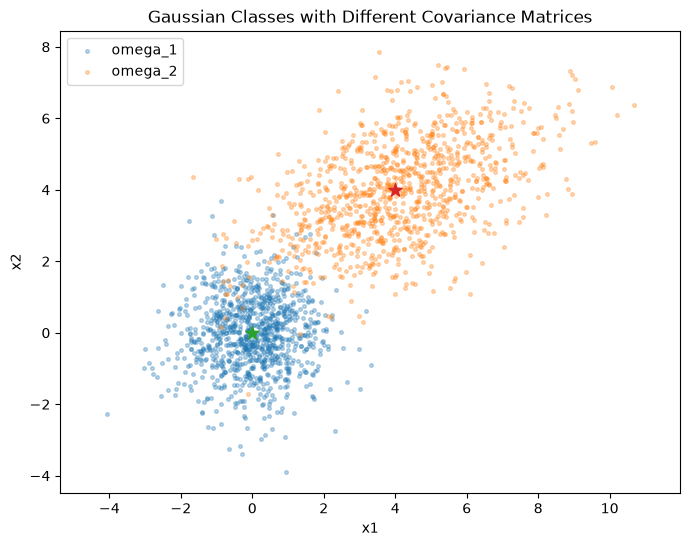
\includegraphics[width=\textwidth]{unequal_covariance_samples.png}
    \caption{Generated class samples.}
  \end{subfigure}
  \hfill
  \begin{subfigure}[t]{0.48\textwidth}
    \centering
    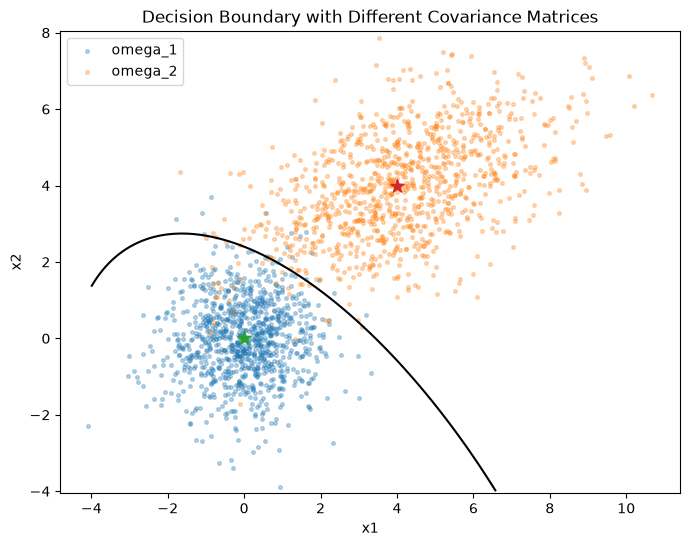
\includegraphics[width=\textwidth]{unequal_covariance_boundary.png}
    \caption{Resulting decision boundary.}
  \end{subfigure}
  \caption{Two Gaussian classes with different covariance matrices.}
  \label{fig:unequal-covariance-classes}
\end{figure}

Here, different classes have different covariance matrices and thus their respective data points have different spread and now that we have different covariance matrices the quadratic term survives in the discrimination function and thus it leads to a quadratic boundary.

\section*{INFERENCE}

After these experiments we came to realize a lot of things like how covariance matrix controls the shape and orientation of the 2D gaussian data and how eigenvalues measures the spread while eigenvector controls the direction and how covariance also controls the boundary geometry when you classify using the discrimination function like linear when you have similar covariance and quadratic when you have different covariance for different classes.

\end{document}
